\chapter{Business Information Visualization of time-oriented Data}
\label{chap:BIV}


\iffalse
\listoftodos

\section{Outline} \todo{Remove from BA}
\begin{enumerate}
    \item The role of InfoVis in Business. Visual Analytics. Selfservice. Insights in Company/ Business. $\Rightarrow$ Business Data
    \subitem But: Other data types also in Business: IoT. Not covered because it is a too wide topic.
    \subitem Business use VA tools to get insight into data.
    \item Need for good visualizations for Business data
    \subitem What are business data? $\Rightarrow$ data types
    \item 2nd challenge: BigData.
    \subitem Where does BigData occur? Application Areas. Streaming Data
    \subitem Is BigData relevant for Business Data? Application Areas of Business Data
    \item Solutions in Literature
    \subitem Aggregation
    \subitem Abstraction
    \item Tools in Business
    \subitem Requirements: Visual Analytics Tools
    \subitem New Visualization Techniques -> Extensionability (p.12, "open
framework fed with pluggable visual and analytical components for analyzing
time-oriented data is useful. Such a framework will be able to support multiple
analysis tasks and data characteristics, which is a goal of Visual Analytics."
\cite{Aigner2007})
    \subitem Market Relevance: Qlik, Tableau
    \subitem Other Approaches: Jaspersoft(because its scalable),
    \subitem Comparison
    \item Conclusion: Which tool for time-oriented data?
\end{enumerate}
\fi
----- \\*


\section{Large Data}
Nowadays, the challenge in BIV is to handle large amounts of data and displaying them in an effective manner. The effective manner was defined by Shneiderman \cite{paterno1997concurtasktrees, Shneiderman2008, Keim2008}: \textit{"Overview first, zoom in and filter, then details on demand}. Overview is a basic yet important task because it navigates the user in the data and allows further analysis.  But as large data appears with a number of challenges creating this overview is more difficult\label{problems}:
\\*
\textit{Overlap}: 
If the whole dataset is visualized or even a subset the data may overlap and reduce visual clutter.
\\*
\textit{Visual Noise}: 
Even if data items are not overlapping data in large data sets might be to similar to each other. Thus, the user cannot differentiate distinct items on the screen.
\\*
\textit{Limited monitor resolution}:
Even if large monitors are used to visualize data in the end the available pixels on the monitor is smaller than the number of data items in a dataset. 
\\*
\textit{Limited visual perception}:
Moreover, human perception is limited.
\\*
\textit{Finding region of interest}:
If the data set is too large and overlap occurs the user faces the challenge of finding an interesting subset in the data.
\\*{Navigation}:
To find a region of interest the user might zoom in. But then another challenge occurs in navigating in the large data set.
\\*
\textit{Information Loss}:
While reducing the number of data items to present them on the limited screen informations in the data can be lost. The important question is which data characteristics to keep such that the user tasks still can be supported.

This is why Shneiderman itself extended its own mantra with the use of aggregation markers and Keim formulated it as \textit{Analyze First - Show the Important - Zoom and Filter, and Analyze Further - Details on Demand}\cite{Keima}. The effective representation of large amounts of data requires to extend the Overview by the use of aggregation which can be achieved by appropriate techniques, correct parametrization, interaction and analytical methods\cite{Aigner2008}. 
\\*
Moreover, visualization of large data sets are limited by two "hardware" restrictions: the \textit{Monitor Resolution} and \textit{Human Perception}.

\subsubsection*{Monitor Resolution}\label{resolution}
Even though large wall-sized screens have been developed nowadays monitors with a display width of 50 cm are used in business. Sometime, -depending on the department- two or three monitors are combined for a larger wall. Thus, the maximum number of pixel which can be used at the workspace ranges from 786.432 (1024x768) to 6.912.000 (3 monitors à 1920x1200).
Concluding, the amount of data in collected data exceeds the maximal number of screen pixels by far. But, besides the monitor resolution human perception is a critical point in limiting the number of pixels.
\\*
\subsubsection*{Human Perception} \label{perception}
% What can humans perceive? How many pixels? 
The brain is limited in perceiving pixels on the screen as well as patterns created by visualizations. Since space in brain is represented different from computer monitor pixels in the brain have a different shape. We call them brain pixels. According to \cite{Ware2012a} brain pixels are nearly represented by ganglion cells. Ganglion cells are neurons which send information to the cortex. In the fovea one ganglion cell cares about one single cone. In the periphery one ganglion cell handles thousand rods and cones. Thus, the brain pixel resolution in the fovea is much higher than in the periphery. 
To model how many data items are percepted by the human brain it is important to make the following distinction: 
\\*
\textit{TBP = total amount of brain pixels which is stimulated by the screen pixels}\\*
and unique stimulated brain pixels: \textit{USBP = TBP - redundant brain pixels}.\\*
USBP are the number of pixel who determines the human perception of data items. A measure of display efficiency (DE) is the ratio of USBP and screen pixels(SP): \textit{DE = USBP/ SP}.

\begin{figure}[H]
    \centering
    \scalebox{.3}{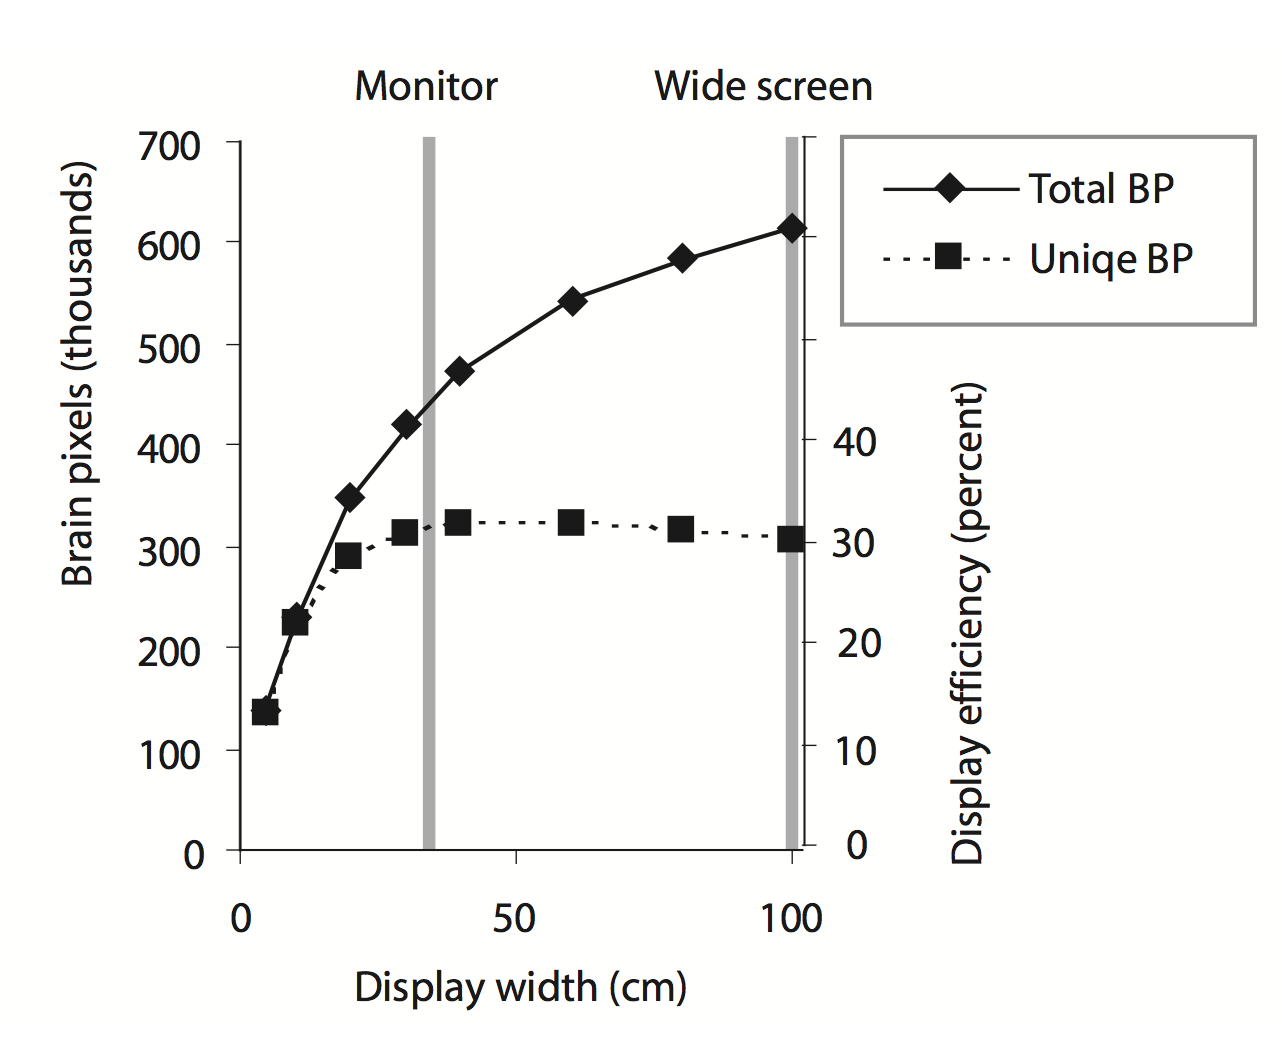
\includegraphics{src/images/DE}}
    \caption{Simulation of display efficiency by exposing the brain to a 1 mio. pixel screen. From \cite{Ware2012a}.}
    \label{fig:DE}
\end{figure}

This shows, that a monitor larger than 40cm wide are not increasing the display efficiency anymore. For large data sets this allows the conclusion that the perception of large data has a limit in the human perception. The current monitor size (which approximately is  40-50cm) is sufficient to respond to the number of USBP.

Talking of TBP  the human visual system is able to perceive 15mio pixels per eye\cite{Deering1998}. Assuming that the amount of perceivable pixels for two eyes is larger than 15mio pixels but smaller than 30mio pixels due to the overlap of the field of view the max. amount of perceivable pixels (pp) is:
\begin{math}
15 mio. \leq pp < 30 mio.
\end{math}

Nevertheless, the important question is not the amount of perceivable pixels but whether the data structure, patterns, trends and further information in the data can be perceived as the human brain is a pattern detection machine\cite{Ware2012a}. If we consider the brains ability to detect patterns aggregation methods for visualizations are not only tolerated but moreover recommended. Moreover, the main concern for visualization techniques should be the perception of patterns: trend, outliers, clusters. 
\\*
\\*
In conclusion, human perception shows that visual scalability of techniques and monitor resolution are not important. The interesting question is whether tools integrate aggregation methods to outline patterns.

% Users in BIV are usually no computer scientist. [Share of Workers in Business] 
% Self-Service Data
% Role of Visual driven analysis -> need for tools








% Data types for Information Visualization
\section{Data type} \label{data}

For choosing appropriate visualization techniques the first step is in understanding the underlying data and creating a correct data model\cite{Aigner2011}, so that the visualization technique represents the underlying data structure and offers best insights\cite{Bacic}. \textit{Aigner et. al.} proposed  the following questions to model the visualization problem: 

\begin{itemize}
    \item What is presented?
    \item Why is it presented?
    \item How it is presented?
\end{itemize}
\textbf{What is presented?}\\*
Talking of large time-oriented data for business we will consider the three given characteristics of the data: characteristics of business data, time-dependency and their size. Business data is collected in many different areas. The following table gives an overview about the applications: 

\begin{table}[th]
	\centering
	% caption format: \caption[<business aplications>]{<long version>}
	\caption[Table 1]{Business applications\cite{Brachman1996,Tegarden1999}}
	\label{businessapplications}
	\begin{tabu}{ll}
	\toprule
	Marketing & Financial Sector \\
	Fraud Detection & Manufacturing and Production \\
	Operations Planning & Market Analysis \\
	Health Care & Network Management\\
	\bottomrule
	\end{tabu}
\end{table}

For each application area exists a number of publications covering different aspects. Thus, the analysis of every single application would go beyond our scope and we decided to consider data with the following characteristics: 
\begin{enumerate}
    \item The data is structured. 
    \item The data is abstract.
    \item The data is multi-variate.
    \item The data is discrete.
\end{enumerate}
\textbf{Structured data}: Data can come in many different forms. Unstructured data appears in text, speech and language processing\cite{Borgo2013}. Structured data comes in tables in which each attribute are represented by one column and each row is one data item. The attributes can be either numerical or text-based. As multi-variate data is usually presented in tables\cite{Borgo2013} we assume that business data is structured.\\*
\textbf{Abstract data}: Abstract data is defined as data without any spatial relationship in the data\cite{Shneiderman1996}. \\*
\textbf{Multi-variate data}: 
Often, multi-variate is mixed-up with the term multi-dimensional. For this reason we define  multi-variate data by the number of dependent attributes. If the dataset holds more than two dependent attributes then we call the data \textit{multi-variate}. In contrast, multi-dimensional depicts the number of independent attributes of a dataset\cite{Aigner2011}.  \\*
\textbf{Discrete and time-oriented data}: A time-oriented dataset contains data items which change over time. Each data item has a timestamp which is saved in one table-column. The time-dependency of the data structures the data by a given order. Every data item is mapped to a specific point in time with a smallest possible unit such as seconds. Time with a smallest unit is mapped to integer\cite{Aigner2011} and thus we assume that time-oriented business data is discrete and has a given order. Ordered discrete data is called \textit{time series}. The time series is an ordered sequence of n data items $T=(t_1+t_2+...+t_n),t_i\in\mathbb{R}$. Thus, we will focus on the analysis of time series data. \\*
These assumptions are based on the work of Tegarden in which business data is described as abstract and multi-variate and discrete\cite{Tegarden1999}.
\\*
\todo{drin lassen? Raus?}
Eventhough, data can be point-based or interval-based (scope), linear or cyclic (arrangement), ordered branching and with multiple perspectives(viewpoint)\cite{Aigner2011}. We will not narrow our focus further but talk on an abstract level. Our perpective is to explore visualization techniques with different scopes, arrangements and viewpoints according to their scalability but of course, every visualization technique is designed for a specific scope such as linearity or seasonal behaviour. The decision for a specific visualization technique is still up to the user. \todo{hier evtl. die unterscheidung von radial und nicht radial einführen / linear oder zyklisch?}.\\*
\textbf{Large data:} Lastely, we characterize the size of the data. Therefore, we stick to a definition of Huber. He devided data in small, medium, large, huge and massive data. Large data according to\cite{Huber1994} is defined as data sets with $10^6$ and huge data with $10^8$ data entries. We are considering large and huge amounts of data. Nowadays, companies strive to do \textit{Big Data}. Big Data in typically defined as data with  high volume, high velocity, high veracity and high variety\cite{Wang2015}. The contribution of our work to Big Data is the study of presentation of of high volume data sets.



% User Tasks
\section{Time-oriented User Tasks} \label{tasks}
\textbf{Why is it presented?}\\*

Every tool for decision-support should consider the user perspective. The business user is a kind of person which is interested in verify existing hypothesis (verification) and discover new patterns (discovery) and by using the tool he expects the tool to assist him in analyzing the data, finding critical points and perform analysis automatically\cite{Brachman1996}. Verification and discovery in the analysis of time-oriented data can be split in seven major tasks\cite{Esling2012}:

\\*
\textbf{T1: Query by Content}
\\*
Query by content describes the retrieval of similar items to the query and returns a set with the most similar solutions to the query. In time-oriented data query by content returns the \textit{k} most similar time series to the queried time series.
\\*
\textbf{T2: Clustering}\\*
Clustering is the process of finding expressive groups (clusters) out of the data. Therefore, the dataset is devided into subgroups according to some similarity measure. In the context of large time-oriented data clustering is important to compare similar time-series.
\\*
\textbf{T3: Classification}\\*
In classification the task is to find the right group the item belongs to. According to \textit{Aigner et al.} temporal classification describes the preprocess of finding the correct group for given data or dataset. This task is important for large data to abstract the data and make them handable. As this task is preprocessing and not data presentation or exploration we will not check whether the tools support the user in this task. 
\\*
\textbf{T4: Segmentation}\\*
Segmentation splits a time series into \textit{k} meaningful subsequences (segments)\cite{batyrshin2007perception}. 
\\*
\textbf{T5: Prediction}\\*
In Prediction\textit{k} future events are predicted based on the past \textit{n} time series. This process is also known as \textit{forecasting}. Forecasting 
\\*
\textbf{T6: Anomaly Detection} \\*
Anomaly detection points out events which behave in a different way than expected.
\\*
\textbf{T7: Pattern Discovery} \}\*
Pattern discovery finds regularly appearing structures in a time series.  It covers the exploration of trends, outliers and clusters. Especially, in business this task is one the most important tasks.\todo{quote finden}


\iffalse
\begin{tikzpicture}[sibling distance=12em,
  every node/.style = {shape=rectangle, 
    draw, align=center,
    top color=white}]]
  \node [shape = ellipse] {Visualization Tasks}
    child { node [shape = ellipse] {visualization methods} %time-oriented data: 
      child { node [shape = ellipse] {right visualization method} }
      child { node [shape = ellipse] {right parametrization} 
        child { node {navigation in time} }
        child { node {search} }
        child { node {comparison} }
        child { node {manipulation} } } }
    child { node [shape = ellipse] {analytical methods} %large time-oriented data: 
      child { node {aligned at}
        child { node {relation sign} }
        child { node {several places} }
        child { node {center} } }
      child { node {first left,\\centered,\\last right} } };
\end{tikzpicture}
\fi

% Visualization Techniques
\section{Visualization of large-scale time-oriented Data} \label{vis}
\textbf{How is it presented?}
% introduction of methodology: selection of vizTechniques, introduction of classes
The following section discusses several visualization techniques for time-oriented data including the question of their scalability because the key to a successful representation of the data is the choice of an appropriate technique. This is shown in the cognitive fit theory\cite{Vessey1991} as this theory showed a significant increase of user task performance the better the visual representation of a problem fitted to the cognitive user model. Visualizations of time-oriented data therefore have to represent the cognitive user model. Based on the findings in literature we assume that the cognitive user model is represented by the user tasks which we described in section \ref{tasks}.\\* 
\textbf{Standard Visualizations of time series data}
Usually time series data is visualized with line charts. However, line charts can only show \textit{univariate} data. Our selection of visualization techniques is based on Aigner et al.\cite{Aigner2011} which presents current approaches to visualize time-oriented data. Hereby, we focus on 34 techniques which can be used to show business data: abstract, multi-variate and discrete data (compare section \ref{data}). 
As the work of Aigner was published in 2011 we completed the set of techniques with current approaches based on the \href{http://survey.timeviz.net/}{TimeVizBrowser}. Moreover, we consider only stand-alone visualization techniques which are techniques no systems, tools or software. In literature a significant amount of publications describe new tools or systems which tackle the visualization of time-oriented data. These tools usually are specific tools which can only be applied in a limited field. As we write this work with the perspective of business users tools have to be generic and single-task systems are not appropriate.

We are aware that this discussion cannot be exhaustive as time-oriented data is a current research area and day-to-day new visualization techniques are developed.
Moreover, time-oriented data appears in different areas of business: E-commerce, Smart Health, E-Government, Science \& Technology, Security \& Public safety. Each sector collects different types of data and uses different applications, which makes it impossible to name every single existing visualization technique.


However, we think that this work gives a good overview of visualization techniques as we stick to Keim's taxonomy\cite{Keim1995} of visualization techniques for multi-variate data which classifies them into the classes: \textit{geometric-projective}, \textit{graph-based}, \textit{hierarchical}, \textit{icon-based} and \textit{pixel-oriented}.
\\*
\textbf{Graph-based} techniques present large graphs by using layout algorithms\cite{Keim1996}.
\\*
\textbf{Geometric projection} techniques (GP-techniques) map multi-dimensional data to the 2D screen\cite{FerreiradeOliveira2003}.
\\*
\textbf{Pixel-oriented} techniques map each data item to one pixel on the screen. Position and color are used to represent data attributes\cite{Keim1996}.



\\*
\textbf{Hierarchical} techniques divide the k-dimensional space into subspaces and shows them hierarchically. 
\\*
\textbf{Icon-based} techniques map each data item onto one icon. The attributes are mapped to different icon features\cite{Keim2001}.

\section{Visual Scalability}\label{scalability}

This work studies how well these techniques scale to large data. To define the ability of visualizations to present large amounts of data we introduce the term \textit{visual scalability}.
Visual or perceptual scalability is defined as the capability of visualization tools in displaying large data sets in an effective manner\cite{Eick2002}. In the context of time-oriented business data effective means the presentation of patterns to support the user tasks. To measure the visual scalability of different visualization techniques for time-oriented data we refer to the work of Eick\cite{Eick2002}. He proposed to measure visual scalability by the database metrics of the dataset and the visual characteristics of the visualization technique. \\*

\textbf{Database metrics} measures the \textit{size of the database} in bytes, the number of rows or the number of attributes at the level of the visualization tool. For multi-dimensional data the \textit{database metrics} are a combination of the number of rows and the attributes. \\*

\textbf{Visualization characteristics} describe the number of elements and attributes presented on the screen, thus measuring how many distinct items a visualization technique can display. This number is measured on the visualization technique level.
\\*
The combination of the database metrics and the visualization characteristics describes the scalability of a visualization tool. Furthermore, the tools scalability is influenced by more factors which will be discussed later (\ref{factors}).

\subsection{Visual Scalability of time-oriented techniques}
In the analysis of the techniques we discovered that time-oriented techniques are covered by only four classes. Thus, we measured the scalability of four classes. 
 Based on this analysis we identified a number of \todo{Anzahl der Techniken einfügen} techniques which are appropriate to show large time-oriented data. These techniques will be described in detail.

\begin{table}[H]
	\centering
	% caption format: \caption[<Scalability of Visualization Classes>]{<long version>}
	\caption{Scalability of Visualization Classes}
	\label{vizScalability}
	\begin{tabu}{  | l | l | l |}
	\toprule
	Visualization Class & Technique & References\\
	\midrule
	    \multirow{10}*{Geometric} 
		& EventRiver        & \cite{Luo2012}\\
		& Flocking Boids    & \cite{Moere2004}\\
		& Intrusion Detection\\
	    & Kiviat Tube       & \cite{Tominski2005}\\
        & Layer Area Graph\\
        & MultiComb         & \cite{Tominski}\\
        & Multi-resolution CircleView & \cite{Keim2005}\\
        & Parallel Glyphs   & \cite{Fanea2005}\\
        & Temporal Star     & \cite{Noirhomme-Fraiture2002}\\
        & TimeWheel         & \cite{Tominski}\\
        & Worm Plots\\ \hline
        \multicolumn{3}{|p{\linewidth}|}{
        \textbf{Geometric projection} techniques (GP-techniques) map multi-dimensional data to the 2D screen\cite{FerreiradeOliveira2003}. The mapping-function often includes data reduction techniques (see section \ref{analytical}). Thus, the visualization characteristics of GP-techniques strongly depend on the mapping-function. When data reduction techniques are involved, this class of techniques becomes a high-potential class for large data sets as they allow to present large to huge data.} \\ \hline
        
		\multirow{3}*{Hierarchical} 
		& Pixel-Oriented Network Visualization \\
		& Software Evolution Analysis & \cite{}\\
		& Timeline Trees \\ \hline
		\multicolumn{3}{|p{\linewidth}|}{\textbf{Hierarchical} techniques: we analyzed three hierarchical visualization techniques. One technique included aggregation techniques by collapsing the nodes. With collapsed nodes the technique can display large to huge amount of data. Pixel-oriented Networks use clustering and thus, can.} \\ \hline
        \multirow{5}*{Icon-based}
        & Gravi++\\
        & InfoBUG\\
        & PeopleGarden\\
        & Spiral Graph\\
        & VIE-VISU\\ \hline
        \multicolumn{3}{|p{\linewidth}|}{
        \textbf{Icon-based} techniques: As every data item requires one icon icon-based techniques can show less data items than the number of pixels on the screen. When showing large data icon-based techniques face the challenge of clutter and occlusion\cite{Borgo2013}. Thus, icon-based techniques can display small- to medium-sized data sets.}\\ \hline
        \multirow{12}*{Pixel-oriented}
        & 3D ThemeRiver & \cite{Imrich2002}\\
        & Braided Graph\\
        & CircleView\\
        & Data Tube Technique\\
        & history flow\\
        & Kaleidomaps\\
        & Pixel-Oriented Network Visualization\\
        & Recursive Pattern\\
        & Spiral Display\\
        & Stacked Graphs\\
        & ThemeRiver\\
        & Time Curves\\
        & TimeRider\\ \hline
        \multicolumn{3}{|p{\linewidth}|}{
        \textbf{Pixel-oriented} techniques: Since only one pixel per data item is used this class can maximize the used screen space. Let $M$ be the monitor resolution with the screen-width $w$ and the screen-height $h$, $P$ the number of pixels in $M$ and $D$ the maximum of data which can be displayed at once. In pixel-oriented techniques  \begin{math}
        D = w*h
        \end{math}
        which shows that pixel-oriented techniques can display large, but not huge data.}
        \\ \hline
	\bottomrule
	\end{tabu}
\end{table}


Most of the existing visualization techniques nowadays still are not appropriate in visualizing large data. Pixel-based visualizations represent each data item by one pixel and thus, are limited to 2 mio. pixels. Even new visualization techniques which where developed to visualize "very large" data sets follow the pixel-oriented approach\cite{Keim1995, Keim1996}. Icon-based visualizations display one data item per icon and thus can display even less data than pixel-oriented visualizaton techniques. The most promising techniques are hierarchical and geometric-projective techniques as they combine aggregation or abstraction with visualization. Their scalability depends on the mapping-function. 
One interesting extension of pixel-oriented techniques is the \textit{multi-resolution} approach\cite{Keim2005}. The idea is to show more relevant data items at a pixel-based level and less relevant data items in an aggregated way. In Multiresolution CircleView recent data is shown at full resolution in the middle of the circle and previous-year-data is placed at the outer circle. With multi-resolution it is possible to extent the pixel-limit from $w*h$ to larger data sets. 

\begin{table}[H]
	\centering
	% caption format: \caption[<Scalability of Visualization Classes>]{<long version>}
	\caption{Scalability of Visualization Classes}
	\label{vizScalability}
	\begin{tabu}{ l | c }
	\toprule
	Visualization Class & Scalability\\
	\midrule
	Geometric &  \cellcolor{green!25 } > 2 mio. pixel\\
	Hierarchical & \cellcolor{green!25} > 2 mio. pixel \\
	Icon-based & \cellcolor{red!25} $\leq$ 1 mio. pixel \\
	Pixel-oriented & \cellcolor{yellow!25} $\leq$ 2 mio. pixel \\	
	\bottomrule
	\end{tabu}
\end{table}





%Aspects of Scalability:
% Wie viele Datenpunkte sind notwendig, um Pattern darzustellen? -> data 
% Interaction Techniques
% Downsampling -> Analytical Methods

 The challenges of large-scale data for ADV are \textit{scalability} and \textit{dynamics}\cite{Wang2015}. With its volume the challenges for large-scale data are also challenges for Big Data defined as high volume, high velocity, high veracity and high variety data sets\cite{Wang2015}. In this work we concentrate on the scalability challenge for visualization techniques. The challenge is in finding appropriate techniques\cite{Aigner2008,Keim2005} which scale to large amount of data.
 
\fi

\subsection{Visualization characteristics of GP-Techniques}
Geometric-projective visualizations seems to be the most scalable visualization technique depending on the mapping function. For this reason we will explore techniques in the geometric-projective class in detail and discuss their scalability.


Furthermore, we suggest to devide GP-techniques into \textit{radial} and \textit{non-radial} visualizations\cite{Diehl2010} as our  analysis has shown that a large part of GP-techniques is based on a radial layout. Radial GP-techniques share common properties such as the maximum number of attributes which is set to 10-20 attributes\cite{Diehl2010}.\\*


\begin{table}[H]
	\centering
	% caption format: \caption[<Radial and non-radial GP-techniques>]{<long version>}
	\caption[Table 1]{Radial and non-radial GP-techniques}
	\label{radialTable}
	\begin{tabu}{lcc}
	\toprule
	GP-Technique & radial & non-radial \\
	\midrule
	Flocking Boids &  & x \\
	Kiviat Tube & x &  \\
	MultiComb & x &  \\
	Multi-resolution CircleView & x &  \\
	Parallel Glyphs & x &  \\
    Temporal Star & x &  \\
	TimeWheel & x & \\
	\bottomrule
	\end{tabu}
\end{table}

As discussed in \ref{scalability} the scalability of visualizations is measured by the number of distinct items.

\textbf{Flocking Boids} \todo{genauer beschreiben} simulate the evolution of data items in 3D. Thus, data objects are represented by a colored, curved line with changing transparency called \textit{boid}.  A data object is an aggregation of same data items, e.g. one boid is one stock market company. A boid calculates the average of multiple data attributes and uses behavior rules to simulate the development of a data object. The rules define the position of data item over time and its velocity. Boids correspond to distinct items on the screen. Thus, the maximum measured number of used boids defines the scalability. Flocking Boids was able to handle 500 boids at a time. Thus the scalability of Flocking Boids is 500 which is low compared to pixel-oriented techniques(2mio items)\cite{Moere2004}. 
Analytical Methods such as clustering or subset selection are outsourced to database algorithms and interaction techniques are not implemented but could be extended\cite{Moere2004}.
\begin{figure}[H]
    \centering
        \scalebox{.3}{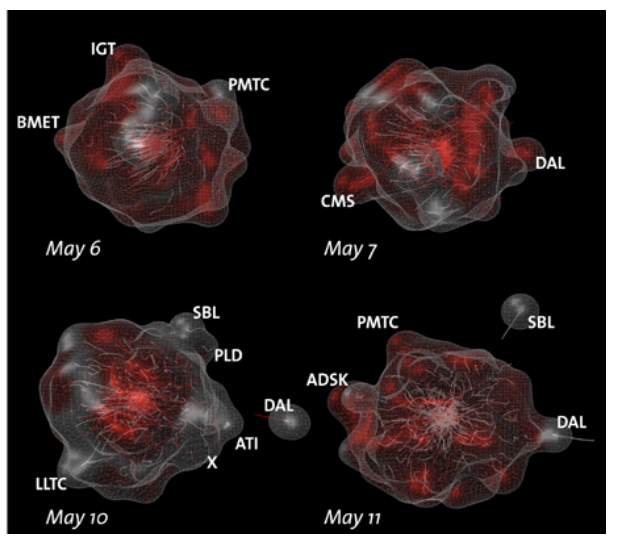
\includegraphics{src/images/FlockingBoids}}
    \caption{Flocking Boids. From \cite{Aigner2011}.}
    \label{fig:flockingboids}
\end{figure}
\\*
\textbf{Kiviat Tube} is a unfolded Radar Chart along the z axis in 3D. Several Radar Charts are stacked behind each other along the time (z) axis and form a tube. Thus, variables are mapped on radial aligned planes and can be compared. Interaction such as changing the planes positions and navigating through time enables the user to compare different variables over time.\\*
The number of attributes is limited to approximately 10-20 attributes as the radial layout limits the number of variables. The number of time-steps 
\begin{figure}[H]
    \centering
        \scalebox{.3}{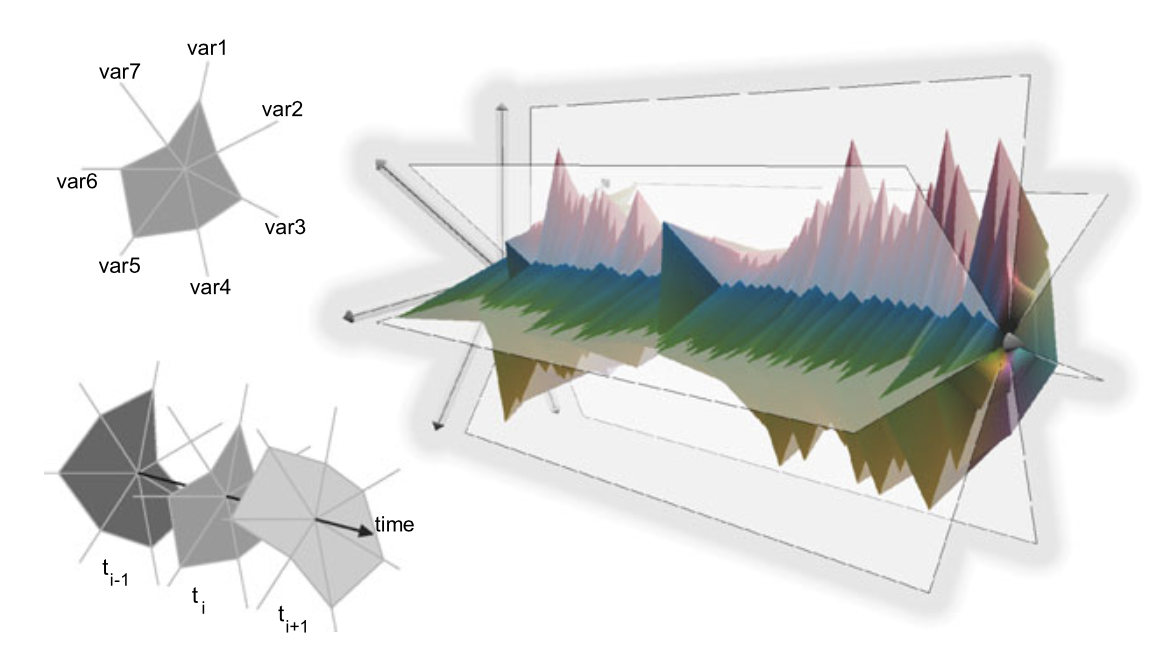
\includegraphics{src/images/KiviatTube}}
    \caption{Kivit Tube. From \cite{Aigner2011}.}
    \label{fig:kiviattube}
\end{figure}
\\*
In \textbf{MultiComb} \textit{k} time series plots are mapped on a circle in two possible ways. One way is to position the plots along the circumference. Or the plots are mapped perpendicular to the circumference. In this option the plot resembles a star.  
\textbf{Multi-Resolution CircleView} extends the CircleView technique by aggregating data according to their relevance. Similar to CircleView the circle is devided in k segments and k is the number of attributes. The least relevent data is placed at the outer circle with a high aggregation level and the most relevant data in the inner circle. The higher the relevance the lower the aggregation level. The number of displayed data items thus depends on the relevance function. 
\begin{figure}[H]
    \centering
        \scalebox{.3}{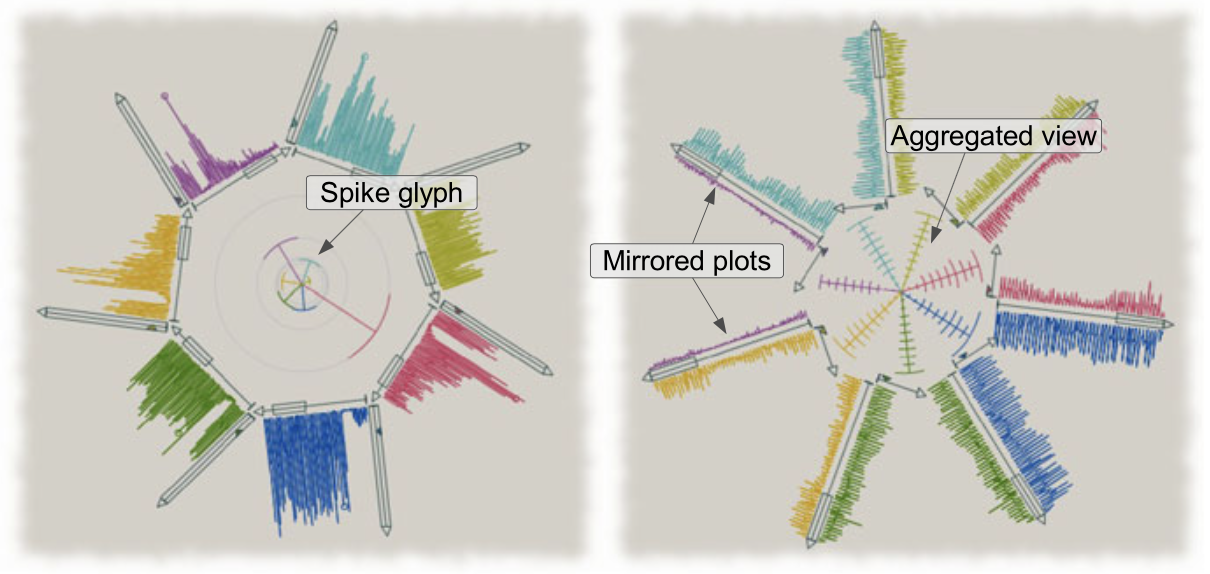
\includegraphics{src/images/MultiComb1,2}}
    \caption{Multi Comb. From \cite{Luo2012}.}
    \label{fig:multicomb}
\end{figure}
\\*
\textbf{Multi-resolution CircleView} enhances the CircleView technique. Instead of mapping each value to one pixel, data items are aggregated. More recent items are placed in the middle of the circle. These items are represented by one pixel each. Less relevant items are aggregated and placed at the outer part of the circle. These items are usually from a preceding point of time.
\begin{figure}[H]
    \centering
        \scalebox{.3}{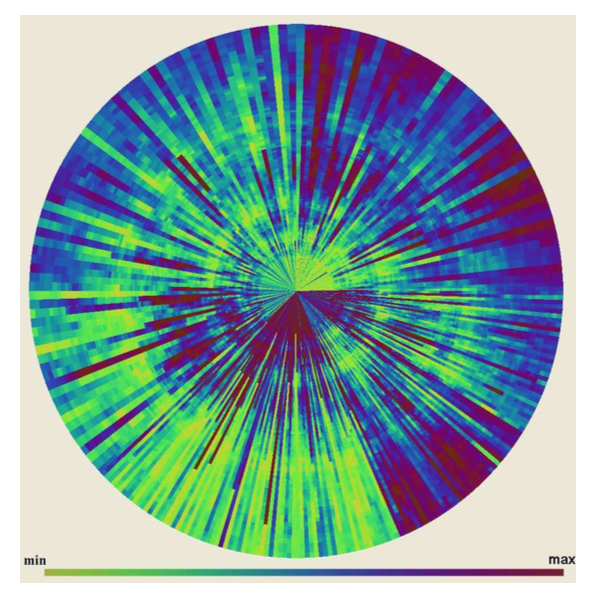
\includegraphics{src/images/MultiResolutionCircleView}}
    \caption{Multi-resolution CircleView. From \cite{Keim2005}.}
    \label{fig:multiresolutioncircleview}
\end{figure}
\\*
\textbf{Parallel Glyphs} pair Parallel Coordinates with Star Glyphs. While similar to Parallel Coordinates each data item is represented by a polyline which connects the vertical axis (attributes) the attribute axis are radially unfolded in 3D and show the data value of the data item over time. Thus, each data value over time is represented by a star glyph. The visualization can be expanded by connection lines over star glyphs. Through the extension of 2D to 3D parallel glyphs are able to display more data rows than parallel coordinates (PC). PC had the problem of clutter while displaying 15.000 data on a gray-scale.  items\cite{Keimb}.
Parallel Glyphs provide brushing of polylines, filtering, axis reordering, rotating in 3 directions, transparency support if the glyphs overlap each other, focus+context presentation through magnification lenses.
\begin{figure}[H]
    \centering
        \scalebox{.3}{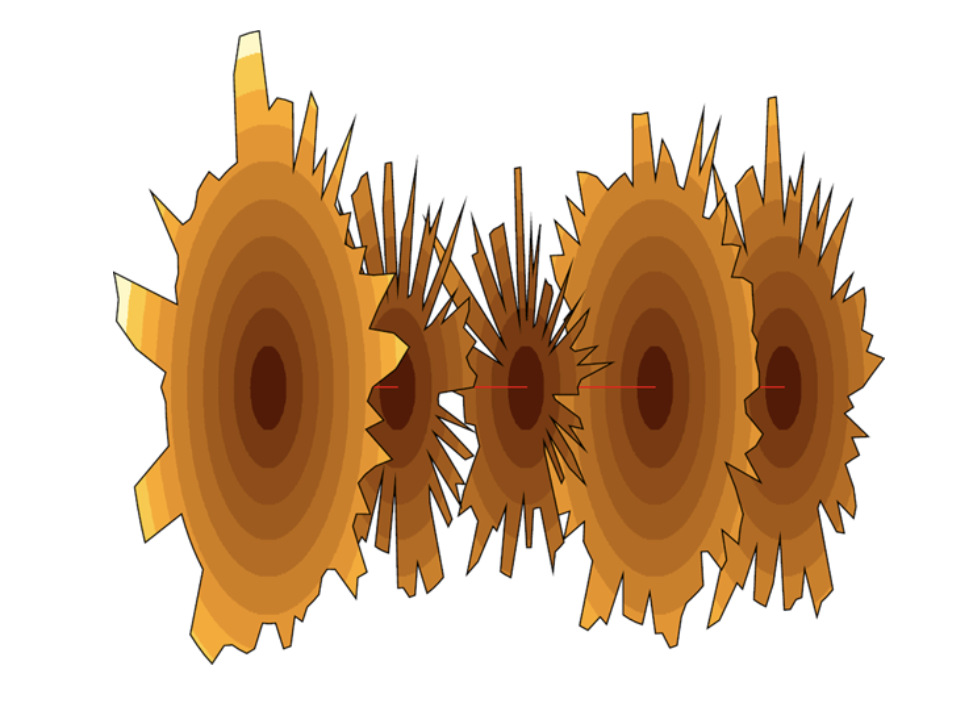
\includegraphics{src/images/ParallelGlyphs}}
    \caption{Parallel Glyphs. From \cite{Aigner2011}.}
    \label{fig:parallelglyphs}
\end{figure}
\\*
\textbf{Temporal Star} aligns multiple attributes in a star-like manner around the centre. Each star is one point of time. The time axis connects several stars to a 3D-object.
\begin{figure}[H]
    \centering
        \scalebox{.3}{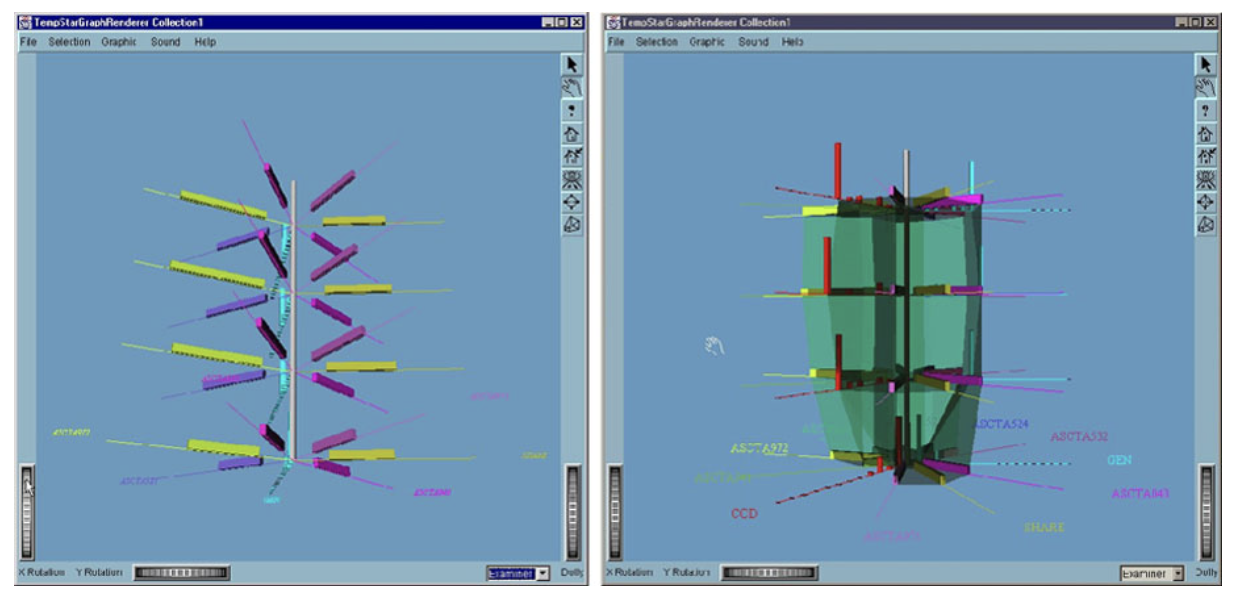
\includegraphics{src/images/TemporalStar}}
    \caption{Temporal Star. From \cite{Aigner2011}.}
    \label{fig:temporalstar}
\end{figure}
\\*
\textbf{TimeWheel} is a 2D technique. Similar to variation one of \textit{MultiComb} attribute axis are positioned along the circle circumference. In the centre of the circle the time axis is placed. 
\begin{figure}[H]
    \centering
        \scalebox{.3}{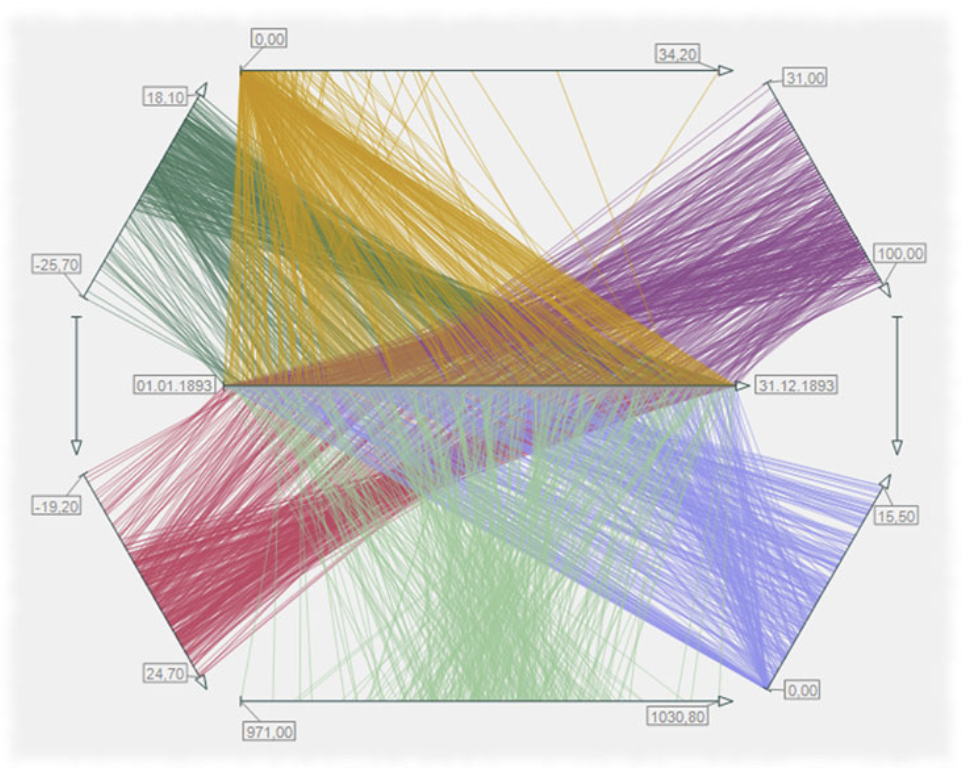
\includegraphics{src/images/TimeWheel}}
    \caption{Time Wheel. From \cite{Aigner2011}.}
    \label{fig:timewheel}
\end{figure}
\\*

\begin{table}[H]
	\centering
	\caption[Table 1]{Scalability of GP-Techniques}
	\label{GPscalability}
	\begin{tabu}{lcc}
	\toprule
	GP-Technique & radial & non-radial \\
	\midrule
	Flocking Boids &  & x \\
	Kiviat Tube & x &  \\
	MultiComb & x &  \\
	Multi-resolution CircleView & x &  \\
	Parallel Glyphs & x &  \\
    Temporal Star & x &  \\
	TimeWheel & x & \\
	\bottomrule
	\end{tabu}
\end{table}


In summary, visualization tools should offer advanced data visualization (ADV) to visualize time-oriented multi-variate data. The term ADV is not unambigiously defined. \textit{Aigner et. al} classify Parallel Coordinates as a standard visualizations\cite{Aigner2011} whereas \textit{Keim et. al.} \cite{Keim} are talking about Parallel Coordinates as a novel techniques. This discussion of course is determined by the time epoche. The longer a visualization technique is known the more it is counted as a standard visualization technique. In our understanding ADV is a visualization technique which is able to scale to large and huge amounts of data.
However, only few techniques are able to represent billions of data. In the end, most of them are limited through the 2D-screen. Factors which enhance the scalability are \textit{improved visual metaphors}, \textit{interaction techniques} and \textit{data reduction}.


\section{Analytical Methods}\label{analytical}
Comparing every visualization technique the need for data reduction becomes obvious. In the literature \textit{data abstraction and aggregation} are well know techniques for data reduction\cite{FerreiradeOliveira2003,Aigner2011, Keim2005}. There exist two ways to data reduction: reduce data horizontally or vertically. 
Vertical data reduction describes the process to remove data rows whereas horizontal data reduction is used for dimensionality reduction. 
\begin{figure}[H]
    \centering
        \scalebox{.1}{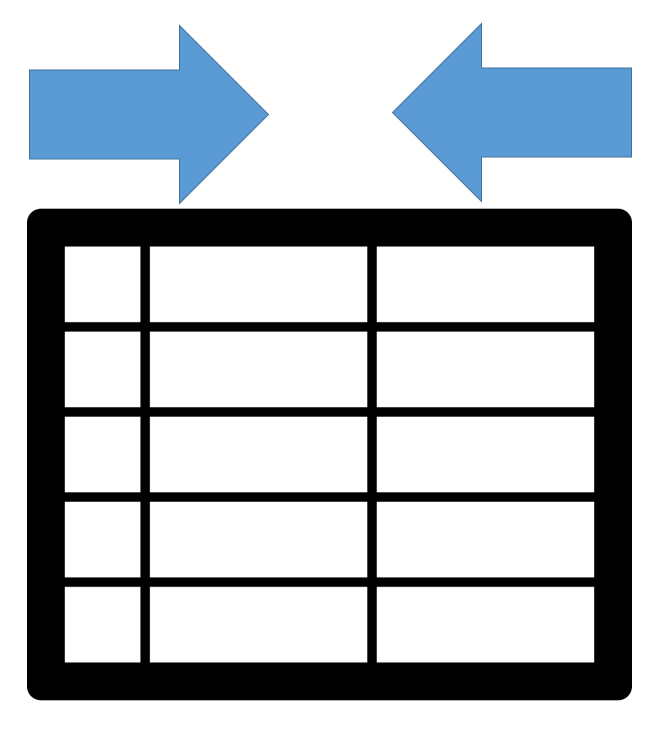
\includegraphics{src/images/dimreduce}}
    \caption{Horizontal Data Reduction}
    \label{fig:my_label}
\end{figure}

\begin{figure}[H]
    \centering
        \scalebox{.1}{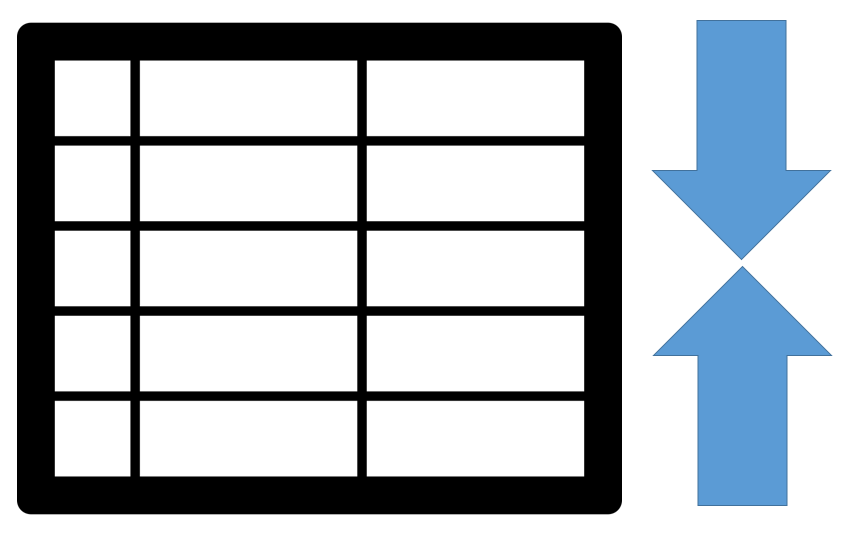
\includegraphics{src/images/aggregation}}
    \caption{Vertical Data Reduction}
    \label{fig:my_label}
\end{figure}

\subsection{Vertical Data Reduction}
One way to decrease the size of large or huge data sets is to remove data rows. This section lists several data removal techniques. One important issue for every technique is the question which data to keep and which data to remove. The disadvantage of data reduction is the information loss.
\subsubsection*{Sampling}
Sampling describes a strategy to reduce data by creating a sample of the original data. Thereby, sampling is scalable, reduces clutter, preserves information of the kept data as well as patterns and trends\cite{PiringerHarald2011}. Still, sampling may eliminate outliers or single data items and does not provide any garantuee to avoid visual overlap. 
\subsubsection*{Filtering}
Filtering is a method to reduce data by some specific criteria. In visualization filtering often is based on user input such as dynamic query sliders. Thereby, filtering can support the user in excluding task-irrelevant data portions and unlike sampling filtering may be appropriate to detect outliers. However, as filtering is based on the exclusion of irrelevant attributes it does not garantuee a specific target size of the data set. In some cases the target size might still be too large. Moreover, filtering also does not garantuee to discriminate distinct data items\cite{PiringerHarald2011}.
\subsubsection*{Temporal Data Abstraction}
Temporal Data Abstraction\cite{Aigner2011} reduces the number of data rows by focusing on relevant concepts, patterns, shapes over time and neglecting irrelevant details. Clusters and summery statistics\cite{PiringerHarald2011} are typical examples for data abstraction. However, the authors found a trade-off between abstraction and accuracy: with low abstraction and a high accuracy there exists the problem of cluttering. 
One way to implement temporal data abstraction is to use natural language processing in visualization tools. The tool \textit{Answerrocket} implemented an NLP-Approach connected with visualization. Another way to achieve data abstraction are unsupervised machine learning methods, such as clustering.
Clustering as defined in the user tasks~\ref{sec:user} has the advantage of reducing visual clutter by displaying the natural groups of the data instead of every single data item. It also preserves pattern and outlier if the similarity measure is appropriate.\\*
Temporal Data Abstraction in tools can be implemented by any method which keeps the characteristic shape and removes data points. 
\subsubsection*{Aggregation}
Aggregation describes the process of grouping several data items together. Hierarchical aggregation builds aggregated data items by forming a tree structure and collapsing the children of a tree\cite{elmqvist2010hierarchical}. Binned aggregation devides data into adjacent bins and combines them for aggregation\cite{Liu2013}. Pixel-aware aggregation clusters pixels according to their screen coordinates\cite{li2016polyspector}. M4 aggregation compresses time series data into a set of equidistant time spans\cite{jugel2014m4}.
As time-oriented data has specific characteristics analytical methods have to consider these peculiarities. One way to reduce data size with respect to the time-specific characteristics is temporal aggregation. Hereby, data is aggregated according to the time unit (day, month, year) in temporal hierarchy levels. Examples for temporal aggregation are hierarchical axis \cite{Chung2014} which enable to navigate in time. \todo{mich damit beschäftigen}
\\*
Other ways to reduce data vertically are binning and pivotization. We will not explain them here in detail as they treat continuous and hierarchical data sets which are beyond our scope in this work. 

\subsection{Horizontal Data Reduction}
Besides data removal datasize can be reduced by decreasing data dimensionality. Since business data often is multi-dimensional but visualization techniques are limited in the number of attributes dimensionality reduction is a way to process data sets in a way that they can be displayed by visualization techniques. 
A common way to map a high-dimensional to a low dimensional space is the Principal Component Analysis (PCA)\cite{Aigner2008}. Other approaches are Multi-Dimensional Scaling or Self-Organizing Maps\cite{PiringerHarald2011}. The advantage is that they keep the distance between two points after the projection. However, the attributes in the low-dimensional space are difficult to understand which makes them unintuitive. To overcome this problem hierarchical dimension reduction has been proposed. \todo{Quellen einfügen + evtl. ausformulieren}
%Segmentation Techniques, Factor Analysis, Multidimensional Scaling, FastMap\cite{FerreiradeOliveira2003} Correlation analysis, Information gain or Statistical methods, Sampling, Clustering or Aggregation\cite{Keim2005}



% 3 Methods for Large Data (Aigner2008)
% 1. Temporal Data Abstraction: VIE-VENT + The Spread
% 2. Data Abstraction for Multivariate Data: PCA
% 3. Data Aggregation



\subsection{More factors} \label{factors}
Moreover, besides the database metrics and the visualization characteristic visual scalability is influenced by six factors: 
\begin{itemize}
    \item Human Perception\cite{Keim2005,Deering1998}
    \item Monitor Resolution 
    \item Visual Metaphors
    \item Interactivity
    \item Data structures and algorithms
    \item Computational infrastructure
\end{itemize}
Human perception and monitor resolution are discussed in \ref{perception} and \ref{resolution}. Data structures and algorithms as well as computational infrastructure will not be discussed in this work as it would go beyond our scope. 

\subsubsection*{Visual Metaphors}
Improved visual metaphors enhance the scalability of visualization techniques\cite{Eick2002}. Let $w$ be the monitor width. If each bar in a bar chart would have the width of one pixel, a bar chart could only visualize  $w$ data items. Thus, the visual metaphor of the bar chart limits the technique how many data items can be mapped at most. One way to improve visual metaphors are \textbf{multi-resolution} metaphors\cite{Keim2005}. The resolution is the ratio of data items to screen pixels, e.g. pixel-oriented visualization maps one data item to one pixel and thus, the resolution is 1:1. Multi-resolution combines several resolution in one technique. Usually, the resolution is lower at \textit{Overview-Level} of a multi-resolution visualization higher at the \textit{Detail-Level}. \textit{CircleView} is one visualization technique with a multi-resolution metaphor.
Multi-resolution can be implemented with aggregation and fish-eye lenses. Fish-eye lenses is one interaction technique (discussed in \ref{interaction}). Aggregation for multi-resolution needs to consider a relevant function. Only a part of data items should be aggregated, while others are not.
Multi-resolution is one important aspect for visualization tools to improve visual scalability.
\\*


\todo{Fokus auf Interaction Techniques für große Datenmengen. Warum sind sie wichtig für große Datenmengen?}
\section{Need for Interaction Techniques}
Interaction Techniques describe how the user can interact with the data. In large data sets interaction overcomes the challenges of overlap, limited screen space, identifying a region of interest and navigation presented in \ref{problems}. Thus, interaction technique enhance visual scalability\cite{Tegarden1999}.

Overlap can be eliminated by filtering and zooming. By reducing the data size with filters and drilling down less elements are presented on the screen and hence, overlap is minimized. One alternative to zooming are multiple linked views.\\*

The screen space is enhanced with \textit{interactive distortion techniques}\cite{mackinlay1991perspective}
The main idea of \textbf{interactive distortion techniques} is to present more relevant data enlarged in the focus while keeping the context by showing less relevant data in a smaller presentation. With this technique distortion technique are not  providing additional pixel to the existing screen pixels but they enhance the screen space metaphor by prioritizing the screen pixels.
Examples are \textit{Bifocal Displays}\cite{Spence1982}, \textit{Fish-eye Views} and \textit{Perspective walls\cite{Keim2005}, \cite{mackinlay1991perspective}}.\\*

Navigation can be supported by linked views and information murals, also known as navigational maps\cite{Jerding1998}. With linked views the user can see different level of detail on one glance and navigate in different level of detail with navigational maps. Navigation also helps in finding a region of interest.

Hereby, we assume that interaction is in responsibility of the visualization tools.

\textbf{Filtering}\\*
With filters a set of variables can be selected and the visualization is only showing the respecting variables.
One way of filtering are dynamic queries. They provide a filter-mechanism by multiple widgets, such as sliders or input fields\cite{Hochheiser2004,Shneiderman2008,Aigner2011}. A specific dynamic query are time-boxes. These boxes are rectangular selection areas which are drawn by the user. The tool then only displays values with a similar pattern to the pattern in the time-boxes.

\textbf{Zooming} is the way of drill down into a data set to a lower level of detail. One special way of zooming is semantic zooming\cite{boulos2003use}. Zooming is one method to achieve \textit{Overview + Detail}.

\textbf{Brushing \& Linking}\\*
The user can select data items on the screen(Brushing) and the respective items are highlighted in every connected window (Linking). Therefore, lasso, rubber-band or rectangular selection enables the user to select groups of data items\cite{tegarden1999, Aigner2011}. In the context of time-oriented data a typical brushing activity is the selection of an smaller time-span to see more details during this period of time. Linked views are also known as coordinated windows.
Brushing \& Linking is one method to achieve \textit{Focus + Context}.

\textbf{Distortion techniques}\\*
All distortion techniques transform the undistorted 2D space by a mathematical function and bring more relevant data points to the focus. \textit{Bifocal Displays}, \textit{Fish-eye Views} (also known as Table and Magnification Lense) and \textit{Perspective walls} differentiate in the way they bend the space. Distortion techniques are good in finding outliers. One disadvantage is that the user might loose the context.
\begin{figure}[H]
    \centering
        \scalebox{.25}{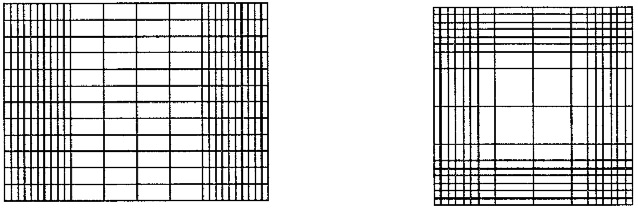
\includegraphics{src/images/f06b}}
    \caption{Bifocal Displays: distortion by linear function. From \cite{Stroe1999}.}
    \label{fig:bifocal}
\end{figure}

\begin{figure}[H]
    \centering
        \scalebox{.25}{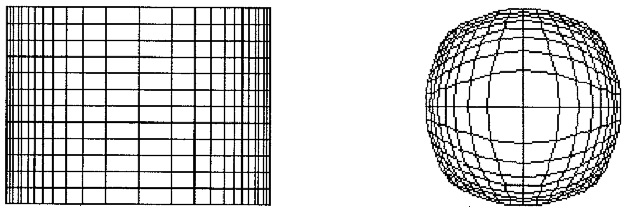
\includegraphics{src/images/f11c}}
    \caption{Fish-eye views:  distortion by a power function with an odd exponent \cite{Stroe1999}.}
    \label{fig:fisheye}
\end{figure}

\begin{figure}[H]
    \centering
        \scalebox{.25}{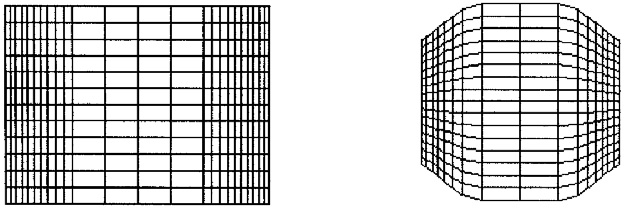
\includegraphics{src/images/f10b}}
    \caption{Perspective Walls: distortion by a half linear and half power function From \cite{Stroe1999}.}
    \label{fig:perspectivewall}
\end{figure}



\textbf{Navigation Maps}\\*
With navigational maps the whole data set is displayed in a miniature version. Usually, navigational maps include linked views in which an enlargened subset of the data is presented. The user can choose the subset which is shown in the linked views with the navigational map.

\textbf{Coarse Presentations}

\section{Layout}
Closely related to interaction techniques is an appropriate layout to enhance visual scalability. Ware\cite{Ware2012} showed that zooming is an easy-to-use-tool for a small amount of items. However, if the user needs to keep three items or more in its visual working memory multiple windows are more effective than zooming. Thus, displaying large time-oriented requires a layout with multiple simultaneous views. Coordinated views are linked views. If one data item is selected and brushed the corresponding characteristic in other windows is also highlighted.
\begin{figure}[H]
    \centering
        \scalebox{.3}{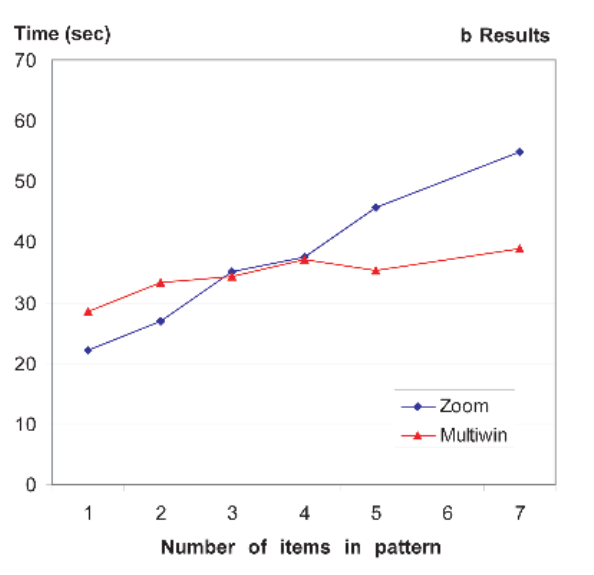
\includegraphics{src/images/zoomVSmultiWindow}}
    \caption{Measured task performance of zooming compared to multiple windows. \cite{Ware2012a}}
    \label{fig:my_label}
\end{figure}
Another layout are \textit{Perspective walls} which is a 3D-representation existing of 3 walls. The front wall shows details and the two side walls provide context. Perspective walls are one method to provide \textit{Focus + Context} and Navigation in large datasets.

\subsection{Visual Scalability 2.0}
After our analysis of the limiting factors for displaying large data sets we come to the conclusion that the limitation by human perception is much higher than the limitation by different visualization techniques. The question is \textit{not} how many pixel can be displayed by a visualization technique but whether the visualization technique allows to percepeive patterns. This is achieved by the \textit{visual metaphor} and \textit{data reduction methods}. Data reduction methods can aggregate overlapping data items to cluster by either mapping data density to color or by displaying the mean and the range of data. Visual Metaphors include techniques such as multi-resolution and thus, enhance the number of pixels which can be displayed. 

\subsection{Factors}
Bringing all findings together, the important factors for visualization of large data sets to support decision-making are the following: 
\begin{enumerate}
\item How advanced visualization techniques are integrated?
\item How data reduction is achieved?
\item How aggregation metaphors are implemented?
\item How pattern perception is supported?
\end{enumerate}

